Our security proof is based on the security proof of NIPoPoWs Suffix Security Proof
under a soft or hard fork. Keep in mind that we operate under the condition of
(1/3)-bounded adversary.\\

The notion of Chain Quality is decisive for the operation of NIPoPoWs under a
velvet fork. Before stepping into the security proof we remind its formal
definition\ref{defn:chain_quality} of this notion and the basic Theorem where its basic metric is computed.\\


\begin{thm}{\textbf{Chain Quality Parameter}}
	In a typical execution the chain quality property holds with parameter $\mu_{cq} > 1 - (1 + \frac{\delta}{2}) \cdot \frac{t}{n-t} - \frac{\delta}{2}$.
\end{thm}
\textit{Proof.} See \cite{Backbone}.\\

Our interest lies in keeping $\mu_{cq} \geq \dfrac{1}{2}$.
From Theorem 3 we have:
\begin{equation*}
	1 - (1 + \frac{\delta}{2}) \cdot \frac{t}{n-t} - \frac{\delta}{2} \geq \dfrac{1}{2} \Rightarrow 
	(1 + \delta)t \leq (1-\delta)(n-t)
\end{equation*}

Thus we have:
\begin{center}
\begin{equation}
	t \leq \dfrac{(1-\delta)}{2}(n - t)
\end{equation}
\end{center}

\begin{thm}{\textbf{Suffix Proofs Security under velvet fork}}
	Assuming honest majority under velvet fork conditions (\ref{defn:velvet_honest_majority}) such that $t \leq (1 - \delta) \dfrac{n_h}{2}$ where $n_h$ the number of upgraded honest players, the non-interactive proofs-of-proof-of-work construction for computable k-stable monotonic suffix-sensitive predicates under velvet fork conditions in a typical execution is secure.
\end{thm}
\textit{Proof.} By contradiction. We follow the proof construction of Theorem \ref{thm:original_suffix_security} 
and extend it. Let $Q$ be a k-stable monotonic suffix-sensitive chain
predicate. Assume NIPoPoWs under velvet fork on $Q$ is insecure. Then, during
an execution at some round  $r_3$, $Q(\mathcal{C})$ is defined and the verifier $V$
disagrees with some honest participant. $V$
communicates with adversary $\mathcal{A}$ and honest prover $B$. The verifier receives
proofs $\pi_\mathcal{A}, \pi_B$ which are of valid structure. Because $B$ is honest, $\pi_B$ is a proof constructed
based on underlying blockchain $\mathcal{C}_B$ (with $\pi_B \subseteq \mathcal{C}_B$), which $B$
has adopted during round $r_3$ at which $\pi_B$ was generated. Consider
$\widetilde{\mathcal{C}}_\mathcal{A}$ the set of blocks defined as
$\widetilde{C}_\mathcal{A} = \pi_\mathcal{A} \cup \{ \bigcup \{\mathcal{C}_h^r\{:b_\mathcal{A}\}:  \forall b_\mathcal{A} \in \pi_\mathcal{A}, \exists h,r : b_\mathcal{A} \in 
\mathcal{C}_{h}^{r}\}  \}$ where $\mathcal{C}_h^r$ the chain 
 that the honest player $h$ has at round $r$.

The verifier outputs $\neg Q(\mathcal{C}_B)$. Thus it is necessary that $\pi_\mathcal{A} \geq \pi_B$.
We show that $\pi_\mathcal{A} \geq \pi_B$ is a negligible event.
Let $b = LCA(\pi_\mathcal{A}, \pi_B)$. Let the levels of comparison decided by the verifier
be $\mu_\mathcal{A}$ and $\mu_B$ respectively. Let $\mu'_B$ be the adequate level of proof
$\pi_B$  with respect to block $b$. Call $\alpha_\mathcal{A} = \pi_\mathcal{A} \uparrow^{\mu_\mathcal{A}}\{b:\}$,
$\alpha'_B = \pi_B \uparrow^{\mu'_B}\{b:\}$.

From Corollary \ref{cor:adversarial_proof_scheme} we have that the adversarial proof 
consists of a smooth interlink subchain followed by a thorny interlink subchain. We will refer to the smooth part of $\alpha_\mathcal{A}$ as $\alpha^{\mathcal{S}}_\mathcal{A}$ and to the thorny part as $\alpha^{\mathcal{T}}_\mathcal{A}$.   

%%%%%%%%   reconsider this paragraph
Our proof construction is based on the following intuition: we show that the competing
suffix proofs can be conceived as consisting of three distinct parts. Each part denotes a specific set of consecutive rounds and is named after the number of blocks existing
in $\alpha_\mathcal{A}$ for that round set. Part $k_1$ stands for the first part of each proof
between blocks $b = LCA(\pi_\mathcal{A}, \pi_B)$ and $b_2 = LCA(\alpha^{\mathcal{S}}_\mathcal{A}, \mathcal{C}_B)$. Now consider that the block following $b_2$ in $\alpha_\mathcal{A}$ is a smooth one. Let's call this block $b'_2$. This means that $b'_2$ does not belong to $\mathcal{C}_B$ but to a forked chain. In this case part $k_2$ stands for the second part of the proofs and refers to the consecutive rounds from block $b_2$ and until
the Common Prefix is established at $\mathcal{C}_B$ for that fork point. In the case that $b'_2$ is a thorny block, then because of Corollary \ref{cor:adversarial_proof_scheme} no more smooth block are included in $\alpha_\mathcal{A}$ and we consider that $k_2 = 0$.
The third and last part, $k_3$, stands for the rest of the blocks in each proof, where $\alpha_\mathcal{A}$ contains only thorny blocks.\\
The above are illustrated, among other, in Parts I, II of Figure \ref{fig:proof_velvet}.

\begin{figure}[h!]
	\begin{center}
		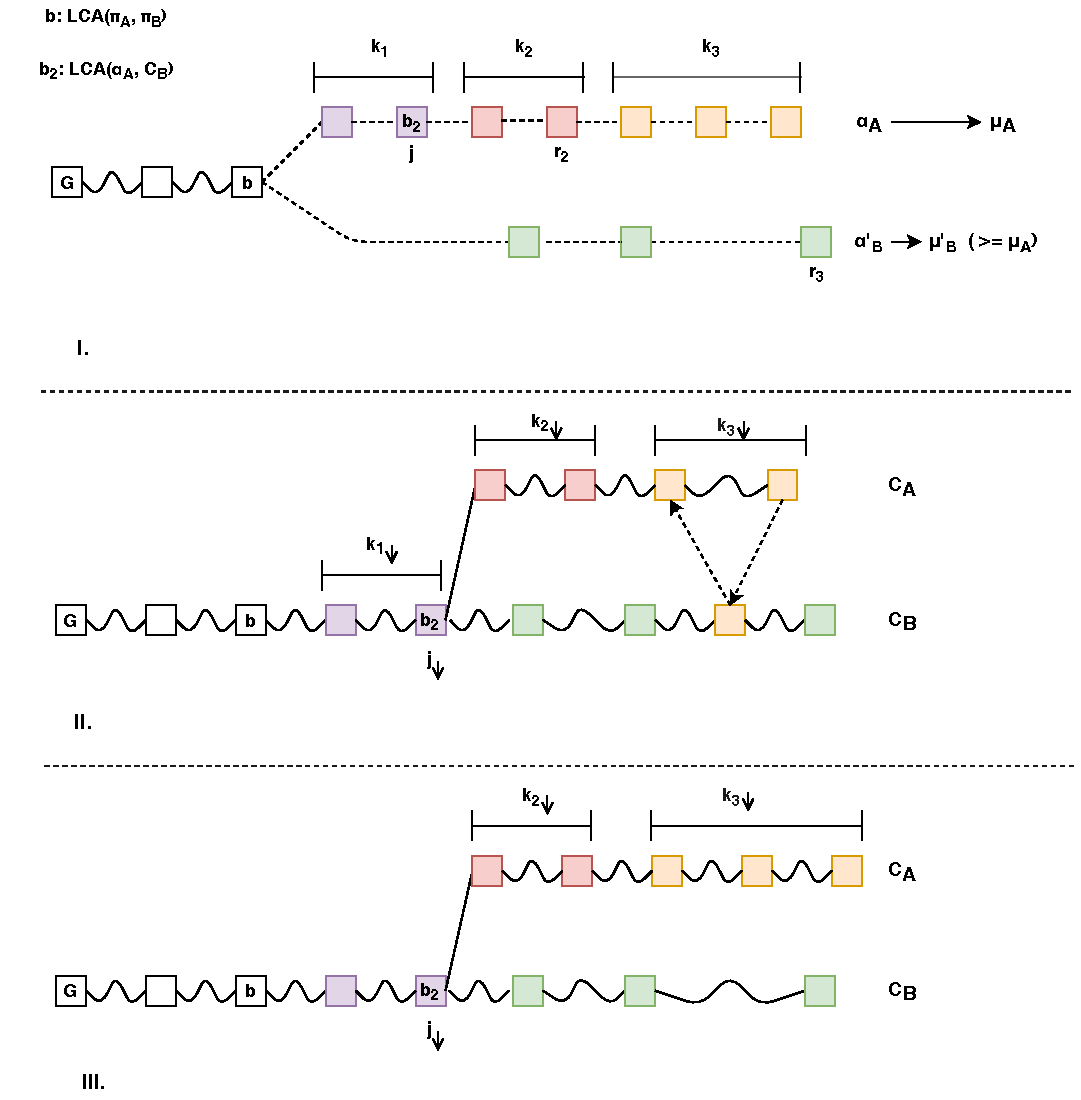
\includegraphics[scale=0.8]{figures/proof_velvet.pdf}
	\end{center}
	\caption{\textit{ Wavy lines imply one or more blocks. Dashed lines and arrows imply
	interlink pointers to superblocks. \textbf{I}: the three round sets in two competing
	proofs at different levels, \textbf{II}: the corresponding 0-level blocks implied by the two proofs,
	\textbf{III}: blocks participating in chain $\mathcal{C}_B$ and block set $\widetilde{\mathcal{C}}_\mathcal{A}$ from the verifier's perspective.}}	
    \label{fig:proof_velvet}
\end{figure}

We will now show three successive claims under velvet fork conditions: First,
$\alpha^{\mathcal{S}}_\mathcal{A}$ and $\alpha'_B \downarrow$ are mostly
disjoint. Second, $a_\mathcal{A}$ contains mostly adversarially generated blocks. And third,
the adversary is able to produce this $a_\mathcal{A}$ with negligible probability.\\
Let $\vert \alpha_\mathcal{A} \vert = k_1 + k_2 + k_3$ and let $k_1, k_2, k_3$ be as defined in the
following Claims.\\
Let round $r_1$ be the round when block $b$ is generated and round $r_2$ when block
$b_2 = LCA(\alpha_\mathcal{A}, \mathcal{C}_B)$ is generated.\\

\textbf{Claim 1:} $\alpha^{\mathcal{S}}_\mathcal{A}$ and
$\alpha'_B\downarrow$ are mostly disjoint. Following the proof of Theorem 
\ref{thm:original_suffix_security} and considering the percentage  of the blocks that contain interlink, we conclude that 
$\vert \alpha^{\mathcal{S}}_\mathcal{A} \cap \alpha'_B\downarrow[1:] \vert \leq k_{1} = g(2^{\mu'_B - \mu_\mathcal{A}})
$, where $g$ the velvet parameter denoting the percentage of upgraded honest parties. 
In order to see this under the velvet fork conditions, first consider that there are no thorny blocks in the adversary's proof between $b$ and $b_2$. This means that if $b_2$ was generated at round $r_{b_2}$ and $\alpha^{\mathcal{S}}_\mathcal{A}[-1]$ in round $r$, then $r \geq r_{b_2}$. In this case Claim 1 of
Theorem \ref{thm:original_suffix_security} applies directly with respect to the velvet parameter $g$. In the opposite case, the adversary includes a thorny block $b_t = \alpha^{\mathcal{T}}_{\mathcal{A}}[0]$ after $b$ and before $b_2$, thus the inequality still
holds and because of Lemma \ref{lemm:thorny_after_thorny} no more honestly generated blocks can be included
in $\alpha_\mathcal{A}$ after $b_t$ and we can immediately proceed to Claim 3 of this proof.

We conclude that there are at least $\vert\alpha_\mathcal{A}\vert - k_1$
blocks after block $b$ in $\alpha_\mathcal{A}$ which are not honestly generated blocks existing in
$\mathcal{C}_B$. In other words, there are $\vert \alpha_\mathcal{A} \vert - k_1$
blocks after block $b$ in $\alpha_\mathcal{A}$, which are either thorny blocks existing in $\mathcal{C}_B$ either don't belong in $\mathcal{C}_B$.\\

\textbf{Claim 2.} 
At least $k_3$ superblocks of $\alpha_\mathcal{A}$ are adversarially generated. Just as
the proof of Theorem \ref{thm:original_suffix_security} and using a similar notation, because of the Common Prefix
property on parameter $k_{2\downarrow}$, $\alpha_\mathcal{A}[k_{1}+k_{2}:]$ could contain
no honestly generated blocks. In order to see this for the velvet fork conditions
let's again consider the case that there is no thorny block in the first
$(k_1 + k_2)$ blocks of $\alpha_\mathcal{A}$ in which case Claim 2 of Theorem 
\ref{thm:original_suffix_security} is immediately applied. In the opposite case,
the adversary includes in her proof a
thorny block at some earlier point. Again, because of Lemma 
\ref{lemm:thorny_after_thorny} the inequality still holds and no more
honestly generated blocks can be included in $\alpha_\mathcal{A}$, so we can proceed to Claim 3
of this proof.\\

%\begin{figure}[h!]
%	\begin{center}
%		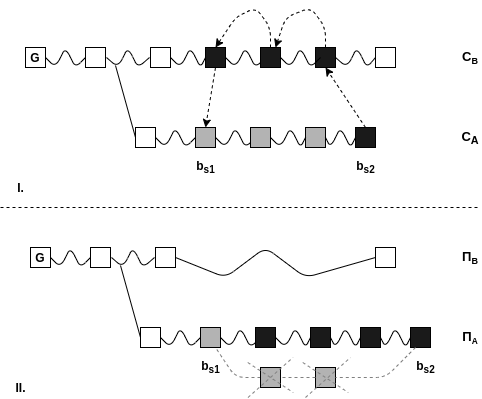
\includegraphics[scale=0.5]{figures/exclude.png}
%	\end{center}
%	\caption{\textit{ Wavy lines imply one or more blocks. Dashed arrows imply interlink 
%pointers to superblocks. Adversarially generated blocks are colored black. Grey colored 
%blocks may be honestly or adversarially generated. \textbf{I}: the 0-level chains, 
%\textbf{II}: the corresponding proof chains; some blocks generated in $C_A$ are excluded 
%from proof $\pi_A$ in favor of the sewed blocks from $C_B$.}}
%	\label{fig:exclude}
%\end{figure}

\textbf{Claim 3.} The adversary may submit a suffix proof such that $\alpha_\mathcal{A} \geq \alpha_B$
with negligible probability.
%%% @TODO: make formal arguments
As argued earlier the last $k_3$ blocks included in $\alpha_\mathcal{A}$ are all thorny blocks. In the worst case  all $k_3 $ blocks
are sewed from $\mathcal{C}_B$. This is the worst case scenario since each adversarially
generated block in $\mathcal{C}_B$ may have dropped one smooth block out of the chain
because of selfish mining. Considering this scenario, because of the strengthened
Honest Majority Assumption for $(1/3)$-bounded adversary, Theorem 3 for Chain
Quality guarantees that the majority of the blocks in $\mathcal{C}_B$ was computed by
honest parties, thus the honestly generated blocks in $\mathcal{C}_B$ for the same round
set sum to more amount of hashing power.\\
From all the above Claims we have that:\\
In the first round set, because of the common underlying chain:
\begin{equation} \label{eq_v_round_set_1}
2^{\mu_\mathcal{A}} \vert \alpha_\mathcal{A}^{k_1} \vert \leq 2^{\mu'_B} \vert \alpha'{_B^{k_1}} \vert
\end{equation}
Because of the adoption by an honest party of chain $\mathcal{C}_B$ at a later round $r_3$, we
have for the second round set:
\begin{equation} \label{eq_v_round_set_2}
2^{\mu_\mathcal{A}} \vert \alpha_\mathcal{A}^{k_2} \vert \leq 2^{\mu'_B} \vert \alpha'{_B^{k_2}} \vert
\end{equation}
In the third round set, because of good Chain Quality under the strengthened Honest
Majority Assumption and Theorem 3 we have:
\begin{equation} \label{eq_v_round_set_3}
2^{\mu_\mathcal{A}} \vert \alpha_\mathcal{A}^{k_3} \vert < 2^{\mu'_B} \vert \alpha'{_B^{k_3}} \vert
\end{equation}
Consequently we have:

\begin{equation*}
2^{\mu_\mathcal{A}} ( \vert \alpha_\mathcal{A}^{k_1} \vert + \vert \alpha_\mathcal{A}^{k_2} \vert + \vert
\alpha_\mathcal{A}^{k_3} \vert ) < 2^{\mu'_B} ( \vert \alpha'{_B^{k_1}} \vert + \vert
\alpha'{_B^{k_2}} \vert + \vert \alpha'{_B^{k_3}} \vert) \Rightarrow
\end{equation*}

\begin{equation} \label{eq_v_all_round_sets}
2^{\mu_\mathcal{A}} \vert \alpha_\mathcal{A} \vert < 2^{\mu'_B} \vert \alpha'{_B} \vert
\end{equation}

Therefore we have proven that $2^{\mu'_B} \vert \pi_B \uparrow^{\mu'_B} \vert >
2^{\mu_\mathcal{A}} \vert \pi_\mathcal{A}^{\mu_\mathcal{A}} \vert$. From the definition of $\mu_B$, we know
that $2^{\mu_B} \vert \pi_B \uparrow^{\mu_B} \vert > 2^{\mu'_B} \vert \pi_B
\uparrow^{\mu'_B} \vert$ because it was chosen $\mu_B$ as level of comparison
by the Verifier. So we conclude that $2^{\mu_B} \vert \pi_B \uparrow^{\mu_B}
\vert > 2^{\mu_\mathcal{A}} \vert \pi_\mathcal{A} \uparrow^{\mu_\mathcal{A}} \vert$.

\begin{flushright}
$\square$
\end{flushright}